\section{MARCO TECNOLÓGICO}

El problema que se busca solucionar en este trabajo tiene relación directa con el campo de estudio de la visión por ordenador. Este campo de la Ingeniería Informática busca, 
a través de sistemas de captación y procesamiento de imágenes, generar información y automatizar procesos con ordenadores. \newline Dentro de este campo se han desarrollado tecnologías que usamos día a día
\cite{szeliskiComputerVisionAlgorithms2022}:

\begin{itemize}
    \item \textbf{\textit{\acrfullr{ocr}}} para realizar reconocimiento de texto en imágenes y documentos.
    \item \textbf{Detección de fallos en maquinaria} en procesos de fabricación.
    \item \textbf{Fotogrametría} para mapear imágenes a modelos 3D.
    \item \textbf{Imagen médica} para uso en operaciones a tiempo real\cite{NEMESIS3DCM}.
    \item \textbf{Detección de objetos} en imágenes o videos.
    \item \textbf{Detección de movimiento} y seguimiento de objetos en escenas.
\end{itemize}

Las aplicaciones que usan herramientas basadas en este tipo de soluciones suelen seguir una estructura similar a la siguiente:

\begin{enumerate}
    \item Capturar información a través de cámaras o flujos de video IP de diferentes características.
    \item (A veces) Realizar un preprocesamiento de las imágenes para adaptarlas al sistema.
    \item Procesar las imágenes para extraer información relevante para el sistema.
    \item Transformar la información extraída a través de algoritmos inteligentes para construir una base de datos que sea útil para el usuario de la aplicación.
\end{enumerate}

En el caso de este trabajo, se tratan problemas de detección de objetos y análisis de cambio. Este tipo de tareas se han llevado a cabo antiguamente a través de algoritmos complejos y deterministas, pero en los últimos 
años, con el auge del aprendizaje automático, se ha creado un nuevo paradigma.

En los siguientes puntos se va a describir de forma breve las técnicas de aprendizaje automático, los sistemas de detección de objetos, seguimiento de cambio y los entornos de desarrollo y despliegue 
de estas técnicas de forma transparente al \textit{Hardware} disponible.
\clearpage

\subsection{Aprendizaje automático y el uso del \textit{Deep Learning}}

El campo del aprendizaje automático busca desarrollar soluciones a través de algoritmos y sistemas que permitan a los ordenadores tratar los datos entrantes como el cerebro humano, siendo capaz de 
generalizar las propiedades que les definen y encontrar patrones.

Este campo tiene su origen en una publicación de Warren McCulloch y Walter Pitts en 1943\cite{mccullochLOGICALCALCULUSIDEAS} en el que presentaban la idea de neurona como una unidad lógica básica 
implementable cuyo estado se puede definir como un "todo o nada", lo cual se representa en el campo de las telecomunicaciones con una función escalón como se ve en la \autoref{fig:Escalon}. Este 
trabajo y diseño de neurona sería conocido más tarde como perceptron.

\begin{figure}[H]
    \centering
    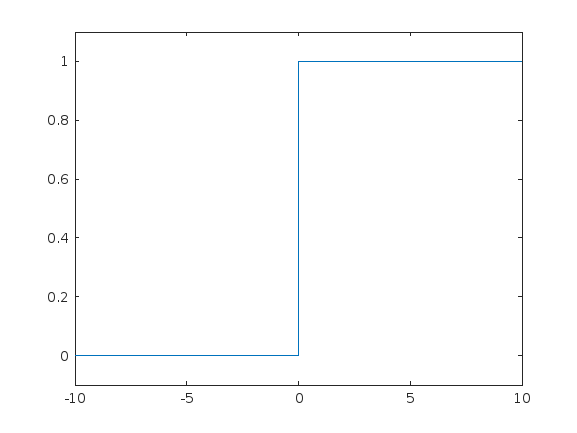
\includegraphics[width=0.4\textwidth]{images/4/Escalon.png}
    \caption{Figura de activación escalón de las primeras neuronas}
    \label{fig:Escalon}
\end{figure}

La estructura básica del perceptron se puede observar en la consiste en un nodo con un número \(\mathcal{N}\) de conexiones entrantes, con unos pesos asociados \(\mathcal{W}\). 
El nodo calcula el sumatorio de cada conexión con su respectivo peso. Al resultado de este cálculo se le añade un factor de \textit{bias} y por último, mediante una función de activación como 
la vista anteriormente, se decide el resultado de salida de la neurona. 

\begin{figure}[H]
    \centering
    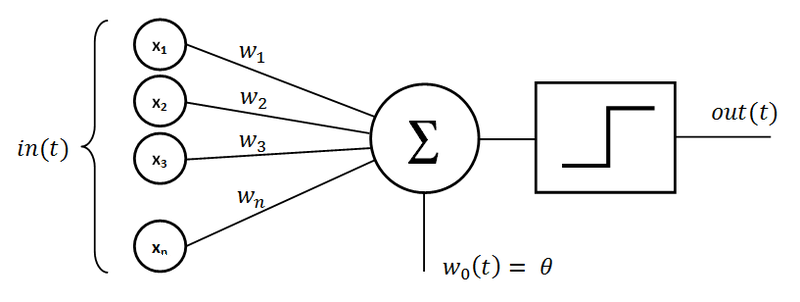
\includegraphics[width=0.5\textwidth]{images/4/perceptron.png}
    \caption{Diagrama general de un perceptron\cite{JgfisherPerceptronPerceptron}}
    \label{fig:Perceptron}
\end{figure}

Más tarde, se conseguiría implementar un diseño electrónico de esta neurona, e interconectar más neuronas entre sí. Estas interconexiones dan lugar a la creación del conecpto de redes neuronales, 
siendo una de las primeras redes complejas de tipo \acrfullr{mlp} (conexión de muchos perceptrones simples).

\subsection{Detección de Objetos}

La detección de objetos como tarea surge de la necesidad de analizar la existencia de objetos en imágenes y; opcionalmente, posicionarlos en las mismas.Para realizar este tipo de tareas se han ido 
desarrollando técnicas tradicionales basadas en algoritmos extremadamente deterministas, pero, con el auge del \textit{Machine Learning}, a partir de 2012\cite{zouObjectDetection202023} 
el paradigma pasó a centrarse en la creación de sistemas detectores basados en \textit{Deep Learning} (Sistemas de Redes Neuronales con una gran cantidad de capas ocultas).

Ambas técnicas se basan en la extracción de características de las imágenes, esto es, la caracterización de imágenes o zonas de interés a través de algoritmos o filtros. Ejemplos de características 
muy usadas que un humano puede entender son:
\begin{itemize}
    \item \textbf{Nitidez} de la imagen aplicando filtros laplacianos como el visto en la \autoref{fig:LaplaceKernel}.
    Con esto nos referimos a x

    hola prueba
    \item Histogramas de color.
    \item Existencia de formas específicas en la imagen.
\end{itemize}

\begin{figure}[H]
    \centering
    \(
    \begin{vmatrix}
        0 & -1 & 0 \\
        -1 & 4 & -1 \\
        0 & -1 & 0
    \end{vmatrix}
    \)
    \caption{Aspecto de un \textit{kernel} de laplace de tamaño \texttt{3x3}}
    \label{fig:LaplaceKernel}
\end{figure}


\subsection{Análisis de cambio}

\subsection{Entornos de desarrollo, sistemas de despliegue y \textit{Hardware} transparente}